\documentclass{ou-report-af}

%\usepackage[subpreambles=true]{standalone}
%\usepackage{import}

\usepackage{microtype}
\usepackage{comment}
% *** GRAPHICS RELATED PACKAGES *** %
\usepackage{graphicx}
% *** PDF, URL AND HYPERLINK PACKAGES ***%
\usepackage{hyperref}
% correct bad hyphenation here %
\hyphenation{op-tical net-works semi-conduc-tor}
% load package for Checkmark symbol: %
\usepackage{bbding}
\usepackage{wrapfig}
\usepackage{amssymb}
%listings
\usepackage{listings}
\usepackage{xcolor}
\usepackage{nameref}
\usepackage{float}
\usepackage{svg}
\usepackage{amsmath}

\definecolor{codegreen}{rgb}{0,0.6,0}
\definecolor{codegray}{rgb}{0.5,0.5,0.5}
\definecolor{codepurple}{rgb}{0.58,0,0.82}
\definecolor{backcolour}{rgb}{0.95,0.95,0.92}

\lstdefinestyle{mystyle}{
    backgroundcolor=\color{backcolour},   
    commentstyle=\color{codegreen},
    keywordstyle=\color{magenta},
    numberstyle=\tiny\color{codegray},
    stringstyle=\color{codepurple},
    basicstyle=\ttfamily\footnotesize,
    breakatwhitespace=false,         
    breaklines=true,                 
    captionpos=b,                    
    keepspaces=true,                 
    numbers=left,                    
    numbersep=5pt,                  
    showspaces=false,                
    showstringspaces=false,
    showtabs=false,                  
    tabsize=2
}
\lstset{style=mystyle}
%end-listings
\usepackage[acronym]{glossaries}
\makeglossaries
\newacronym{sut}{SUT}{System Under Test}
\newacronym{gui}{GUI}{Graphical User Interface}
\newacronym{api}{API}{Application Programming Interface}
\newacronym{vaf}{VAF-SE}{SE Graduation assignment preparation}
\newacronym{big}{Wet-BIG}{Wet op de beroepen in de individuele gezondheidszorg}
\newacronym{cibg}{CIBG}{Centraal Informatiepunt Beroepen Gezondheidszorg}
\newacronym{zorro}{BIG-registration System}{ZOrgverlener Registratie Requirements Ontwikkeling}
\newacronym{alm}{ALM}{Application Lifecycle Management}
\newacronym{gdpr}{GDPR}{General Data Protection Regulation}
\newacronym{vws}{VWS}{Ministry of Health, Wellbeing and Sports}
\newacronym{ind}{IND}{Immigration and Naturalization Service}
\newacronym{indigo}{INDiGO}{INDiGO}
\newacronym{bpm}{BPM}{Business process Management}
\newacronym{sig}{SIG}{Software Improvement Group}
\newacronym{hcp}{HCP}{health care person}

\graphicspath{ {./04_images/} }

\citestyle{agu}

% Dit template is gemaakt door P.J. Molijn in het kader van zijn afstuderen aan de OU in 2014.
% Waarvoor hartelijk dank.
% Minieme maar belangrijke wijzigingen zijn aangebracht door E.M. van Doorn
% Het template is versimpeld door Sylvia Stuurman, 2019.

\usepackage[]{multibib}
\newcites{NonPub}{Non-published Readings}

\usepackage{afterpage}
\newcommand\myemptypage{
    \null
    \thispagestyle{empty}
    \addtocounter{page}{-1}
    \newpage
    }
\usepackage{titling}

\begin{document}
\pagenumbering{roman} % to prevent that the title page will be referred as page 1, which will give the warning that there is a page 1 twice.
\pagestyle{plain}
\title{Using relational algebra in designing public healthcare registers} 
\begin{comment}
Gebruik van relatie algebra bij het ontwerpen van volkgezondheidsregisters
\end{comment}
\author{Gerard Edelaar}

\begin{titlepage}

\begin{center}

%% Insert the OU logo at the bottom of the page.
\begin{tikzpicture}[remember picture,overlay]
    \node at (current page.south)[anchor=south,inner sep=0pt]{
        
\includegraphics[scale=0.7]{./00_common/02_cover/logo}
    };
\end{tikzpicture}

%% Extra whitespace at the top.
\vspace*{2\bigskipamount}

%% Print the title in specific color.
{\makeatletter
%\titlestyle\color{ou-cyan}\Huge\@title
\titlestyle\color{red}\Huge\@title
\makeatother}

%% Print the optional subtitle in black.
{\makeatletter
\ifx\@subtitle\undefined\else
    \bigskip
    \titlefont\titleshape\LARGE\@subtitle
\fi
\makeatother}

\bigskip
\bigskip

by
%door

\bigskip
\bigskip

%% Print the name of the author.
{\makeatletter
\titlefont\Large\bfseries\@author
\makeatother}


\bigskip
\bigskip



\bigskip
\bigskip


\begin{tabular}{lll}
%% Add additional information here, per faculty requirements, e.g
    Student ID number: & 836016215 \\
    Date of presentation: & 14 April 2022\\
    
\end{tabular}

\begin{figure}[htp]
    \centering
    
\includegraphics[width=0.8\textwidth]{./00_common/04_images/ampersand.jpg}
    \label{fig:Ampersand}
\end{figure}

\bigskip


\bigskip

\end{center}

\end{titlepage} 

\myemptypage
\begin{tabular}{lll}
%% Add additional information here, per faculty requirements, e.g
    Title of thesis: & \thetitle  \\
    Student name: & \theauthor \\
    Student ID number: & 836016215 \\
    Date of presentation: & 14 April 2022\\
    Graduation committee: 
        & chair: prof. dr. ir. Stef Joosten \\
        & primary supervisor: dr. Bastiaan Heeren \\
    Degree programme: 
        & Open University of the Netherlands,\\
        & Faculty of Management, Science and Technology \\
        & Master's Programme in Software Engineering \\
    Course code: & \textsc{IM}9703\\

\end{tabular}


\newpage

\tableofcontents
\newpage

\pagenumbering{arabic} % to prevent that the title page will be referred as page 1, which will give the warning that there is a page 1 twice.

\let\cleardoublepage\clearpage

\newpage
\section*{Summary} \label{Summary}
\addcontentsline{toc}{section}{Summary}
\subsection*{Dutch}

In deze thesis gaan we de bruikbaarheid van Ampersand onderzoeken door het ontwerpen van een register systeem bij een overheidsorganisatie.
Ampersand wordt niet breed gebruikt en we vragen ons af waarom dat het geval is en het onderzoek richt zich op mogelijke oorzaken hiervan.

Het doel van Ampersand is om business analisten te helpen correcte informatiesystemen te leveren~\footnote{\url{https://ampersandtarski.gitbook.io/documentation/why-ampersand}}. 
Correct betekent dat het systeem aantoonbaar voldoet aan de regels van de bedrijfsvoering en in ons onderzoek is dat de \acrshort{big}.

Het \acrshort{cibg} is een uitvoeringsorganisatie van het Ministerie van Volksgezondheid, Welzijn en Sport. 
Deze organisatie, waar ik werkzaam ben, beheert register systemen.
Een register systeem, ook wel register genoemd, heeft voor ons altijd een wettelijke basis. 
Dus op basis van een wet, creëert het \acrshort{cibg} een register.
Om dit onderzoek uit voeren hebben we een authentieke case genomen.
Het systeem dat de \acrshort{big} ondersteunt staat op nominatie om vervangen te worden.
De gekozen methode om het onderzoek uit te voeren is dan ook \acrshort{ar}.

Tijdens het ontwerp proces zijn observaties over het verloop van de Ampersand analyse vastgelegd. 
Ook zaken van Ampersand die opvallen zijn meegenomen.
De \acrlong{ca} is opgeleverd en als onderwerp besproken met geïnterviewde personen.

Alle observaties en interviews zijn middels content analyse gerubriceerd en hebben de basis gevormd voor de beantwoording van de hoofd- en subvragen. 
Deze hebben geleid tot het trekken van conclusies op de vraag of Ampersand bruikbaar is voor het ontwerpen van register systemen bij een overheidsorganisatie.
Het is hierbij opgevallen dat register systemen niet anders zijn dan andere informatie systemen.
Het grote verschil is dat een register systeem een wettelijk basis heeft en een informatiesysteem niet per definitie.
De bruikbaarheid van Ampersand om een wet te analyseren is goed, echter moet een organisatie bereid zijn om het te gebruiken. 
Verbeteringen zijn mogelijk op het gebied van documentatie en er kan nog onderzoek plaatsvinden naar het gebruik van tooling om ontwikkeling te versnellen. 


\newpage
\subsection*{English}
In this thesis we will investigate the usefulness of Ampersand by designing a registry system at a government organization.
Ampersand is not widely used and we wonder why that is the case and the research focuses on possible causes of this.

Ampersand its goal is to help business analysts deliver correct information systems~\footnote{\url{https://ampersandtarski.gitbook.io/documentation/why-ampersand}}. 
Correct means that the system demonstrably complies with the rules of business operations and in our research this is the \acrshort{big}.

The \acrshort{cibg} is an implementing organization of the Ministry of Health, Welfare and Sport.
This organization, where I work, manages registry systems.
A register system, also known as a register, always has a legal basis for us.
So based on a law, the \acrshort{cibg} creates a register.
To carry out this research, we have taken an authentic case.
The system that supports the \acrshort{big} is nominated to be replaced.
The chosen method to carry out the research is \acrshort{ar}.

During the design process, observations about the course of the Ampersand analysis were recorded.
Also items of Ampersand that stand out are included.
The \acrlong{ca} has been delivered and discussed as a topic with interviewees.

All observations and interviews have been classified by means of content analysis and have formed the basis for answering the main and sub questions.
These have led to conclusions about whether Ampersand can be used for designing registry systems in a government organization.
It has been noticed that registry systems are no different from other information systems.
The big difference is that a register system has a legal basis and an information system not by definition.
Ampersand its utility for analyzing a law is good, but an organization must be willing to use it.
Improvements are possible in the area of documentation and research can still be done on the use of tooling to accelerate development.
\subsection{Design method} \label{design_method}
The method used in this study is the Ampersand method.
The Ampersand method is based on relational algebra.
Ampersand makes it possible to make a conceptual analysis of problems. The data model created thereby makes it possible to accelerate implementation.


\subsubsection{Relation Algebra} \label{relation_algebra}
The field of the relation algebra, founded by De Morgan, focuses on operations with sets.
The signature item of relational algebra is the relationship, as the name implies.
This relationship has several properties, namely the attributes.
The attributes in the example of \acrshort{big} would be the surname, first names, gender, date of birth, nationality and address of the person concerned and the number and time of registration~\footnote{\acrlong{big} article 3, paragraph 2}.
In addition, the relationship consists of tuples.
Since the relationship is always between two objects, this is called 2-tuples.
The tuples contain the attributes of the relation.

Basically the operations on sets are the following:
\begin{itemize}
    \item Union, $R \cup S$ %vereniging
    \item Intersection, $R \cap S$ %doorsnede
    \item Difference, $R - S$ or $S - R$ %verschil
\end{itemize}
A distinction must be made between relation algebra and relational algebra.
Ampersand uses relation algebra, so is tuple related and the relational algebra is the foundation of e.g. relational databases.
This includes projections, selections and joins.
The latter are therefore not part of relation algebra.


\subsubsection{Ampersand} \label{ampersand}
Ampersand is based on relation algebra and focuses on business rules~\citepNonPub{wedemeijer_l_joosten_smm_michels_garkenbout_jlc_werkboek_ontwerpen_met_bedrijfsregelspdf_nodate}.
Ampersand supplies correct information systems.
In this case, Ampersand's goal is to provide a correct registry system.
Ampersand's other strengths are its support for conceptual analysis.
It is a platform for reactive programming and generates prototypes.
Ampersand describes the goals rather than the steps.

Business rules are there to pursue a common goal.
These rules are converted into an information system. 
The Ampersand method ensures that when a precise set of rules has been established, an information system can be generated. 
Ampersand focuses on business rules.
To learn how Ampersand works in real life, we design a registry in Ampersand that implements the \acrshort{big}~\citepNonPub{van_wet_2018} .

\begin{wrapfigure} {r}{0.52\textwidth} 
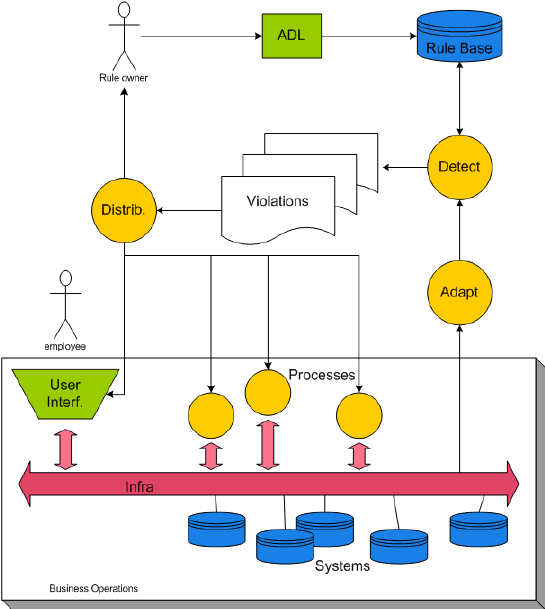
\includegraphics[width=7cm, height=6cm]{Principle-of-rule-based-process-management.png}
\caption{rule-based-proces}
\label{fig:rule-based-proces}
\end{wrapfigure}


The principle of rule-based \acrfull{bpm} as mentioned in \citepNonPub{joosten_joosten} is that any violation of a business rule may be used to trigger actions. 
This is described in the section \nameref{reactive_approach}.

Ampersand consists of concepts that in turn consist of atoms.
An atom is an implementation of the concept.
Inside the \acrshort{big} is a concept "beroep" with associated atoms like "arts, tandarts, etc".
The concepts are given a name, and the name must be recognized by the business.
This also applies to the definition and purpose of the concepts.
These attributes are not mandatory, but when one wants to generate a functional design, these descriptions of the attributes are very useful.
\begin{lstlisting}[language=Octave] 
CONCEPT Beroep "Beroep van een persoon zoals bedoeld in de wet" 
PURPOSE CONCEPT Beroep 
{+Beroep dat uitgeoefend wordt+}
POPULATION Beroep CONTAINS [
    "arts",
    "tandarts",
    "apotheker",
    "gezondheidszorgpsycholoog",
    "psychotherapeut",
    "fysiotherapeut",
    "verloskundige",
    "verpleegkundige",
    "physician assistant",
    "orthopedagoog-generalist"
]
\end{lstlisting}

Concepts can have relationships with each other.
If the data of the concepts is true and the rules yield consistent data then the relationships between real data are facts.
These facts together form one truth.
Not all concepts are directly related.
Within the domain of the \acrshort{big} we could distinguish the concept of "registratie" and the concept of "beroep".
This name is also referred to within ~\citeNonPub{van_wet_2018} in article 3 of \acrshort{big}.
Even the name of the relationship is mentioned in this article, which the legislator calls a "beroepsbeoefenaar".
The law requires that data of the "registratie" be recorded, indicating the corresponding profession (beroep).
In Ampersand, this is modelled as follows.
On the one hand, the "beroep" and also the concept "registratie".
\begin{lstlisting}[language=Octave] 
    CONCEPT Registratie "De registratie van een persoon binnen het register" 
    PURPOSE CONCEPT Registratie 
    {+Vastlegging in het register geeft toegang tot uitoefenen taak binnen de gezondheidszorg+}
\end{lstlisting}
Between the "registratie" and the $persoon$ exists the relationship "beroepsbeoefenaar".
\begin{lstlisting}[language=Octave] 
RELATION beroepsbeoefenaar [Persoon*Registratie] 
MEANING "geregistreerd persoon"
POPULATION beroepsbeoefenaar CONTAINS 
[
  ("Piet",1);
  ("Susan",2);
  ("Gerard",3);
  ("John",4)
]\end{lstlisting}
Also adding the concepts of $persoon$ and $handeling$.
Persons may perform the medical actions, but only when they are qualified.
\begin{lstlisting}[language=Octave] 
    CONCEPT Persoon "Persoon die werkzaam wilt zijn binnen de zorg"
    PURPOSE CONCEPT Persoon 
    {+Vastleggen van de identiteit van de persoon+}
\end{lstlisting}
\begin{lstlisting}[language=Octave] 
    CONCEPT Handeling "Acties die uitgevoerd worden" 
    PURPOSE CONCEPT Handeling 
    {+Vastleggen van de mogelijke handelingen die uitgevoerd kunnen worden binnen de zorg+}
\end{lstlisting}
These concepts can lead us to the following scheme.
\begin{figure}[H] 
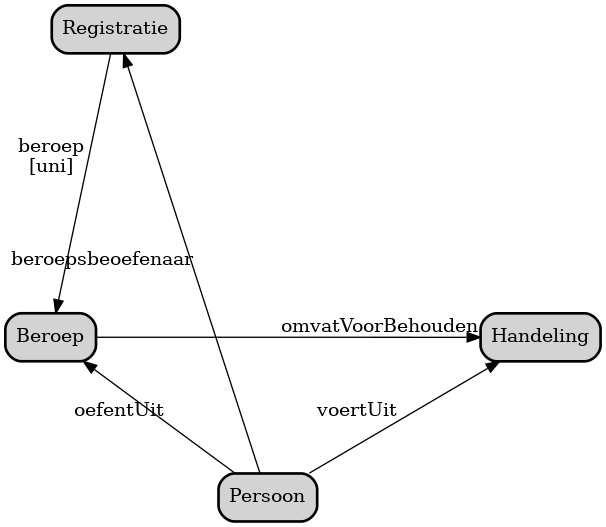
\includegraphics[scale=0.4]{CDConceptBeroep.png}
\centering
\caption{relations}
\label{fig:relations}
\end{figure}
The multiplicity must also be determined for each relation.
\begin{table}[h!]
    \begin{tabular}{||l | l||} 
     \hline
    function & The corresponding control question for the above relation $voerUit$ is\\
    \hline\hline
        Univalent & For each $Persoon$ there is at most 1 $Handeling$\\ %elke P max 1 H
        Total & For each $Persoon$ there is at least 1 $Handeling$ \\ %elke P minimaal 1 H
        Injective & For each $Handeling$ there is only 1 $Persoon$\\ %elke H max 1 P 
        Surjection & For each $Handeling$ there is at least 1 $Persoon$\\ %elke H minimaal 1 P
    \end{tabular}
    \caption{multiplicity}
    \label{tab:multiplicity}
\end{table}

By modelling using the Ampersand method, the question can be answered whether Ampersand provides more insight into the relationships.
As part of the research question, Ampersand can help you gain insight into the relationships.
Although you have to recognize and define these yourself, Ampersand will be helpful in generating functional design and prototype.
The generated prototype will validate the named constraints.
This will prevent registrations that do not meet the constraints.
These constraints are laid down in rules within Ampersand.
For example, a rule can be drawn up that determines whether a person is allowed to perform a certain action.
In figure \ref{fig:relations} the relations are named.
It was previously established that there are 2-tuple relationships.
Here we use the following notation:"$\mathit{relation [Concept \times Concept]}$".
\begin{center}
$\mathit{voertUit [Persoon \times Handeling]}$ ; 
 $\mathit{omvatVoorBehouden [Beroep \times Handeling]~\smallsmile}$
\newline $\subseteq$
\newline $\mathit{beroepsbeoefenaar [persoon \times registratie]}$ ;
$\mathit{beroep [registratie \times beroep]}$
\end{center}
The compared sets are
\newline $\mathit{[Persoon \times Beroep]}$
\newline The rule then will determine if the previous equation is true.
\newline If this is the case, then the rule is validated, otherwise the violation message occurs.
\begin{lstlisting}
    RULE HandelingDoorPersoon: voertUit; omvatVoorBehouden[Beroep*Handeling]~ |- beroepsbeoefenaar; beroep
    MEANING "Een persoon mag handelingen uitvoeren wanneer hij een bepaald beroep uitoefend"
    MESSAGE "Geen toegestane handeling."
    VIOLATION (TXT "Persoon ", SRC I, TXT " voert de handeling uit ", TGT I, TXT " die niet tot zijn beroep behoren ", SRC I[Persoon];oefentUit)
\end{lstlisting}


\subsection{Reactive approach} \label{reactive_approach}

The start of the reactive approach started with the reactive manifesto~\citepNonPub{reactive_manifesto}.
This defines the aspects that a reactive system should meet.
This includes Responsive, Resilient, Elastic and Message Driven.
These are systems that are flexible, loosely coupled and scalable and that makes them easier to develop and maintain.
Reactive Systems are made highly responsive and provide interactive feedback.
\begin{figure}[H] 
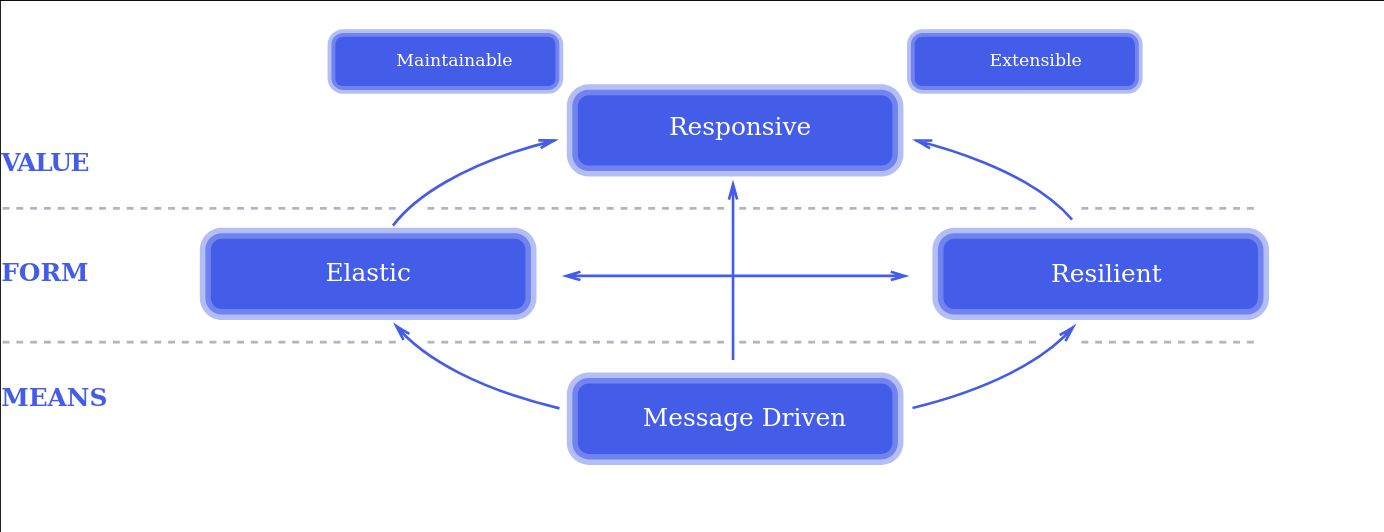
\includegraphics[scale=0.3]{reactive_manifesto.png}
\centering
\caption{reactive manifesto}
\label{fig:reactive manifesto}
\end{figure}


Ampersand is a form of Functional Reactive Programming (FRP)~\citep{elliott_functional_1997}.
The basic of reactive programming is the fact that it involves asynchronous communication.
This means that, as the \citeNonPub{reactive_manifesto} prescribes, use is made of message driven systems, but Ampersand is more than a message-driven system.
It is actually an event-driven system.
The glossary of the \citeNonPub{reactive_manifesto} indicates the difference between message driven systems and event driven systems.
An event-driven system targets event-bus while a message-driven system targets recipients~\citep{bainomugisha_survey_2013}.
The essence is that the order of the flow cannot be determined in advance.
The system will respond to events caused by constraints, Ampersand determines a dynamic flow~\citep{joosten_relation_2018}.




\subsubsection{Law analysis} \label{law_analysis}
The tax authorities have developed a method that is intended to analyse tax laws and other laws.
This is performed in these 6 steps:
\begin{enumerate}
    \item Determining the work area.
    \item Making the structure visible in legislation.
    \item Defining the meaning of legislation.
    \item Validate the analysis results.
    \item Identify missing execution policy.
    \item Setting up the knowledge model.
\end{enumerate}
Emphasis is placed on the cooperation between the implementer, ICT and policy.
By going through the method step by step, one arrives at a shared language.
This shared language includes the definition of concepts by the collaborating parties.
An important part of the approach is dividing the law into small pieces and always refer to these pieces of law in the implementation.
As a result, the method meets the requirement of the justification of government decisions.
The decisions are traceable, explainable, and it is possible to account for them.
What is not clear from the webinar~\citeNonPub{belastingdienst_webinar_2021} is how these steps were converted into an implementation.
The book~\citeNonPub{ausems_wetsanalyse_2021} indicates that the legal analysis method does not contain a development tool, but that the Tax and Customs Administration has developed an instrument based on the legal model, which is not freely available.

\subsection{Design method} \label{design_method}
The method used in this study is the Ampersand method.
The Ampersand method is based on relational algebra.
Ampersand makes it possible to make a conceptual analysis of problems. The data model created thereby makes it possible to accelerate implementation.


\subsubsection{Relation Algebra} \label{relation_algebra}
The field of the relation algebra, founded by De Morgan, focuses on operations with sets.
The signature item of relational algebra is the relationship, as the name implies.
This relationship has several properties, namely the attributes.
The attributes in the example of \acrshort{big} would be the surname, first names, gender, date of birth, nationality and address of the person concerned and the number and time of registration~\footnote{\acrlong{big} article 3, paragraph 2}.
In addition, the relationship consists of tuples.
Since the relationship is always between two objects, this is called 2-tuples.
The tuples contain the attributes of the relation.

Basically the operations on sets are the following:
\begin{itemize}
    \item Union, $R \cup S$ %vereniging
    \item Intersection, $R \cap S$ %doorsnede
    \item Difference, $R - S$ or $S - R$ %verschil
\end{itemize}
A distinction must be made between relation algebra and relational algebra.
Ampersand uses relation algebra, so is tuple related and the relational algebra is the foundation of e.g. relational databases.
This includes projections, selections and joins.
The latter are therefore not part of relation algebra.


\subsubsection{Ampersand} \label{ampersand}
Ampersand is based on relation algebra and focuses on business rules~\citepNonPub{wedemeijer_l_joosten_smm_michels_garkenbout_jlc_werkboek_ontwerpen_met_bedrijfsregelspdf_nodate}.
Ampersand supplies correct information systems.
In this case, Ampersand's goal is to provide a correct registry system.
Ampersand's other strengths are its support for conceptual analysis.
It is a platform for reactive programming and generates prototypes.
Ampersand describes the goals rather than the steps.

Business rules are there to pursue a common goal.
These rules are converted into an information system. 
The Ampersand method ensures that when a precise set of rules has been established, an information system can be generated. 
Ampersand focuses on business rules.
To learn how Ampersand works in real life, we design a registry in Ampersand that implements the \acrshort{big}~\citepNonPub{van_wet_2018} .

\begin{wrapfigure} {r}{0.52\textwidth} 
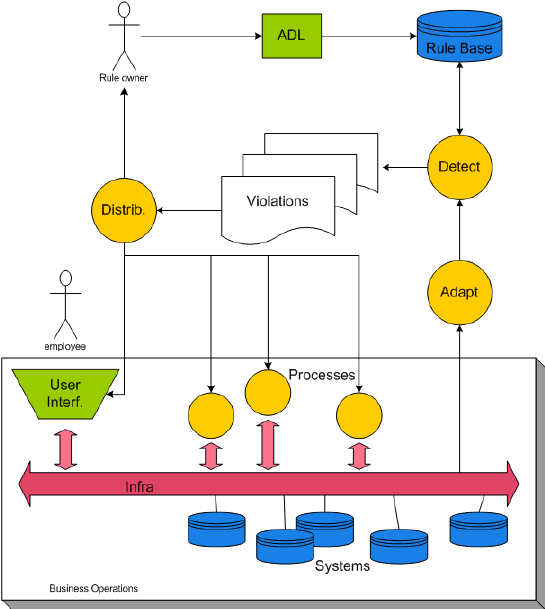
\includegraphics[width=7cm, height=6cm]{Principle-of-rule-based-process-management.png}
\caption{rule-based-proces}
\label{fig:rule-based-proces}
\end{wrapfigure}


The principle of rule-based \acrfull{bpm} as mentioned in \citepNonPub{joosten_joosten} is that any violation of a business rule may be used to trigger actions. 
This is described in the section \nameref{reactive_approach}.

Ampersand consists of concepts that in turn consist of atoms.
An atom is an implementation of the concept.
Inside the \acrshort{big} is a concept "beroep" with associated atoms like "arts, tandarts, etc".
The concepts are given a name, and the name must be recognized by the business.
This also applies to the definition and purpose of the concepts.
These attributes are not mandatory, but when one wants to generate a functional design, these descriptions of the attributes are very useful.
\begin{lstlisting}[language=Octave] 
CONCEPT Beroep "Beroep van een persoon zoals bedoeld in de wet" 
PURPOSE CONCEPT Beroep 
{+Beroep dat uitgeoefend wordt+}
POPULATION Beroep CONTAINS [
    "arts",
    "tandarts",
    "apotheker",
    "gezondheidszorgpsycholoog",
    "psychotherapeut",
    "fysiotherapeut",
    "verloskundige",
    "verpleegkundige",
    "physician assistant",
    "orthopedagoog-generalist"
]
\end{lstlisting}

Concepts can have relationships with each other.
If the data of the concepts is true and the rules yield consistent data then the relationships between real data are facts.
These facts together form one truth.
Not all concepts are directly related.
Within the domain of the \acrshort{big} we could distinguish the concept of "registratie" and the concept of "beroep".
This name is also referred to within ~\citeNonPub{van_wet_2018} in article 3 of \acrshort{big}.
Even the name of the relationship is mentioned in this article, which the legislator calls a "beroepsbeoefenaar".
The law requires that data of the "registratie" be recorded, indicating the corresponding profession (beroep).
In Ampersand, this is modelled as follows.
On the one hand, the "beroep" and also the concept "registratie".
\begin{lstlisting}[language=Octave] 
    CONCEPT Registratie "De registratie van een persoon binnen het register" 
    PURPOSE CONCEPT Registratie 
    {+Vastlegging in het register geeft toegang tot uitoefenen taak binnen de gezondheidszorg+}
\end{lstlisting}
Between the "registratie" and the $persoon$ exists the relationship "beroepsbeoefenaar".
\begin{lstlisting}[language=Octave] 
RELATION beroepsbeoefenaar [Persoon*Registratie] 
MEANING "geregistreerd persoon"
POPULATION beroepsbeoefenaar CONTAINS 
[
  ("Piet",1);
  ("Susan",2);
  ("Gerard",3);
  ("John",4)
]\end{lstlisting}
Also adding the concepts of $persoon$ and $handeling$.
Persons may perform the medical actions, but only when they are qualified.
\begin{lstlisting}[language=Octave] 
    CONCEPT Persoon "Persoon die werkzaam wilt zijn binnen de zorg"
    PURPOSE CONCEPT Persoon 
    {+Vastleggen van de identiteit van de persoon+}
\end{lstlisting}
\begin{lstlisting}[language=Octave] 
    CONCEPT Handeling "Acties die uitgevoerd worden" 
    PURPOSE CONCEPT Handeling 
    {+Vastleggen van de mogelijke handelingen die uitgevoerd kunnen worden binnen de zorg+}
\end{lstlisting}
These concepts can lead us to the following scheme.
\begin{figure}[H] 
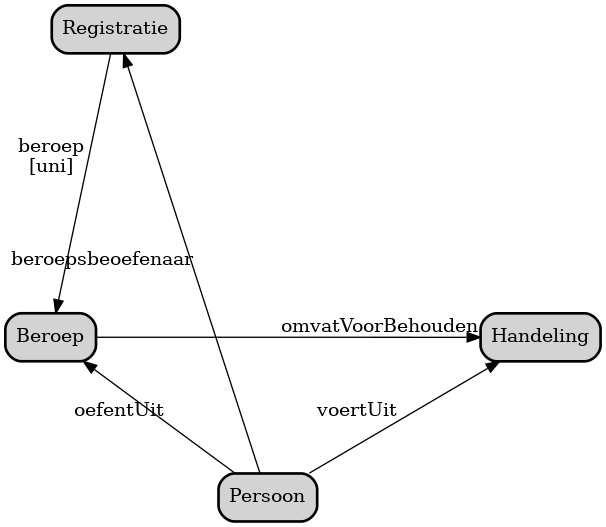
\includegraphics[scale=0.4]{CDConceptBeroep.png}
\centering
\caption{relations}
\label{fig:relations}
\end{figure}
The multiplicity must also be determined for each relation.
\begin{table}[h!]
    \begin{tabular}{||l | l||} 
     \hline
    function & The corresponding control question for the above relation $voerUit$ is\\
    \hline\hline
        Univalent & For each $Persoon$ there is at most 1 $Handeling$\\ %elke P max 1 H
        Total & For each $Persoon$ there is at least 1 $Handeling$ \\ %elke P minimaal 1 H
        Injective & For each $Handeling$ there is only 1 $Persoon$\\ %elke H max 1 P 
        Surjection & For each $Handeling$ there is at least 1 $Persoon$\\ %elke H minimaal 1 P
    \end{tabular}
    \caption{multiplicity}
    \label{tab:multiplicity}
\end{table}

By modelling using the Ampersand method, the question can be answered whether Ampersand provides more insight into the relationships.
As part of the research question, Ampersand can help you gain insight into the relationships.
Although you have to recognize and define these yourself, Ampersand will be helpful in generating functional design and prototype.
The generated prototype will validate the named constraints.
This will prevent registrations that do not meet the constraints.
These constraints are laid down in rules within Ampersand.
For example, a rule can be drawn up that determines whether a person is allowed to perform a certain action.
In figure \ref{fig:relations} the relations are named.
It was previously established that there are 2-tuple relationships.
Here we use the following notation:"$\mathit{relation [Concept \times Concept]}$".
\begin{center}
$\mathit{voertUit [Persoon \times Handeling]}$ ; 
 $\mathit{omvatVoorBehouden [Beroep \times Handeling]~\smallsmile}$
\newline $\subseteq$
\newline $\mathit{beroepsbeoefenaar [persoon \times registratie]}$ ;
$\mathit{beroep [registratie \times beroep]}$
\end{center}
The compared sets are
\newline $\mathit{[Persoon \times Beroep]}$
\newline The rule then will determine if the previous equation is true.
\newline If this is the case, then the rule is validated, otherwise the violation message occurs.
\begin{lstlisting}
    RULE HandelingDoorPersoon: voertUit; omvatVoorBehouden[Beroep*Handeling]~ |- beroepsbeoefenaar; beroep
    MEANING "Een persoon mag handelingen uitvoeren wanneer hij een bepaald beroep uitoefend"
    MESSAGE "Geen toegestane handeling."
    VIOLATION (TXT "Persoon ", SRC I, TXT " voert de handeling uit ", TGT I, TXT " die niet tot zijn beroep behoren ", SRC I[Persoon];oefentUit)
\end{lstlisting}


\subsection{Reactive approach} \label{reactive_approach}

The start of the reactive approach started with the reactive manifesto~\citepNonPub{reactive_manifesto}.
This defines the aspects that a reactive system should meet.
This includes Responsive, Resilient, Elastic and Message Driven.
These are systems that are flexible, loosely coupled and scalable and that makes them easier to develop and maintain.
Reactive Systems are made highly responsive and provide interactive feedback.
\begin{figure}[H] 
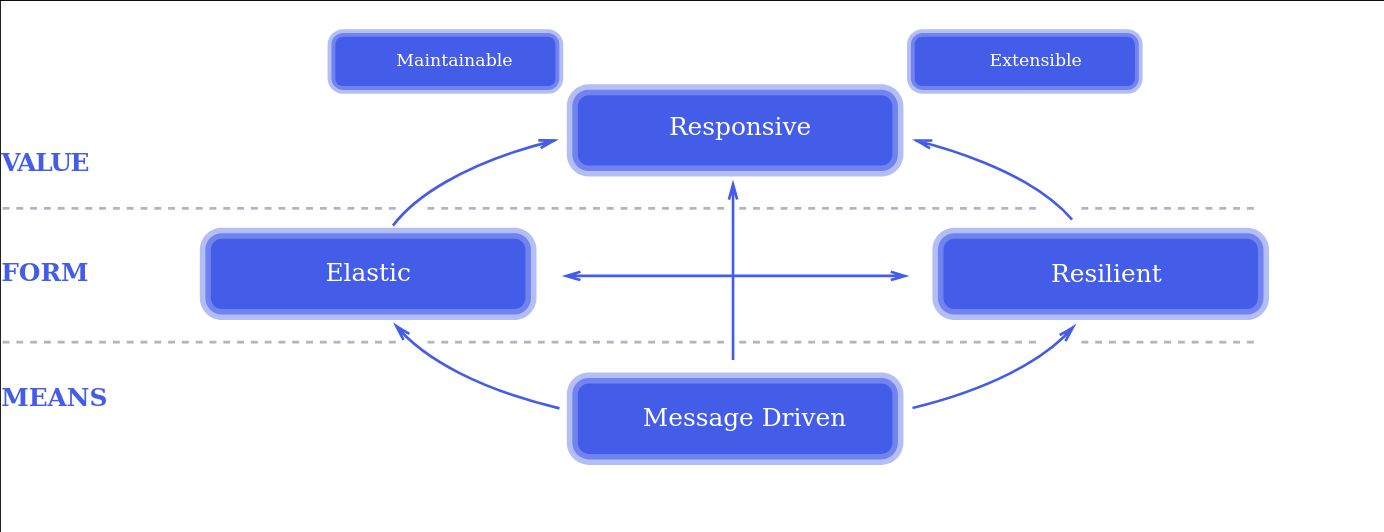
\includegraphics[scale=0.3]{reactive_manifesto.png}
\centering
\caption{reactive manifesto}
\label{fig:reactive manifesto}
\end{figure}


Ampersand is a form of Functional Reactive Programming (FRP)~\citep{elliott_functional_1997}.
The basic of reactive programming is the fact that it involves asynchronous communication.
This means that, as the \citeNonPub{reactive_manifesto} prescribes, use is made of message driven systems, but Ampersand is more than a message-driven system.
It is actually an event-driven system.
The glossary of the \citeNonPub{reactive_manifesto} indicates the difference between message driven systems and event driven systems.
An event-driven system targets event-bus while a message-driven system targets recipients~\citep{bainomugisha_survey_2013}.
The essence is that the order of the flow cannot be determined in advance.
The system will respond to events caused by constraints, Ampersand determines a dynamic flow~\citep{joosten_relation_2018}.




\subsubsection{Law analysis} \label{law_analysis}
The tax authorities have developed a method that is intended to analyse tax laws and other laws.
This is performed in these 6 steps:
\begin{enumerate}
    \item Determining the work area.
    \item Making the structure visible in legislation.
    \item Defining the meaning of legislation.
    \item Validate the analysis results.
    \item Identify missing execution policy.
    \item Setting up the knowledge model.
\end{enumerate}
Emphasis is placed on the cooperation between the implementer, ICT and policy.
By going through the method step by step, one arrives at a shared language.
This shared language includes the definition of concepts by the collaborating parties.
An important part of the approach is dividing the law into small pieces and always refer to these pieces of law in the implementation.
As a result, the method meets the requirement of the justification of government decisions.
The decisions are traceable, explainable, and it is possible to account for them.
What is not clear from the webinar~\citeNonPub{belastingdienst_webinar_2021} is how these steps were converted into an implementation.
The book~\citeNonPub{ausems_wetsanalyse_2021} indicates that the legal analysis method does not contain a development tool, but that the Tax and Customs Administration has developed an instrument based on the legal model, which is not freely available.
\subsection{Design method} \label{design_method}
The method used in this study is the Ampersand method.
The Ampersand method is based on relational algebra.
Ampersand makes it possible to make a conceptual analysis of problems. The data model created thereby makes it possible to accelerate implementation.


\subsubsection{Relation Algebra} \label{relation_algebra}
The field of the relation algebra, founded by De Morgan, focuses on operations with sets.
The signature item of relational algebra is the relationship, as the name implies.
This relationship has several properties, namely the attributes.
The attributes in the example of \acrshort{big} would be the surname, first names, gender, date of birth, nationality and address of the person concerned and the number and time of registration~\footnote{\acrlong{big} article 3, paragraph 2}.
In addition, the relationship consists of tuples.
Since the relationship is always between two objects, this is called 2-tuples.
The tuples contain the attributes of the relation.

Basically the operations on sets are the following:
\begin{itemize}
    \item Union, $R \cup S$ %vereniging
    \item Intersection, $R \cap S$ %doorsnede
    \item Difference, $R - S$ or $S - R$ %verschil
\end{itemize}
A distinction must be made between relation algebra and relational algebra.
Ampersand uses relation algebra, so is tuple related and the relational algebra is the foundation of e.g. relational databases.
This includes projections, selections and joins.
The latter are therefore not part of relation algebra.


\subsubsection{Ampersand} \label{ampersand}
Ampersand is based on relation algebra and focuses on business rules~\citepNonPub{wedemeijer_l_joosten_smm_michels_garkenbout_jlc_werkboek_ontwerpen_met_bedrijfsregelspdf_nodate}.
Ampersand supplies correct information systems.
In this case, Ampersand's goal is to provide a correct registry system.
Ampersand's other strengths are its support for conceptual analysis.
It is a platform for reactive programming and generates prototypes.
Ampersand describes the goals rather than the steps.

Business rules are there to pursue a common goal.
These rules are converted into an information system. 
The Ampersand method ensures that when a precise set of rules has been established, an information system can be generated. 
Ampersand focuses on business rules.
To learn how Ampersand works in real life, we design a registry in Ampersand that implements the \acrshort{big}~\citepNonPub{van_wet_2018} .

\begin{wrapfigure} {r}{0.52\textwidth} 
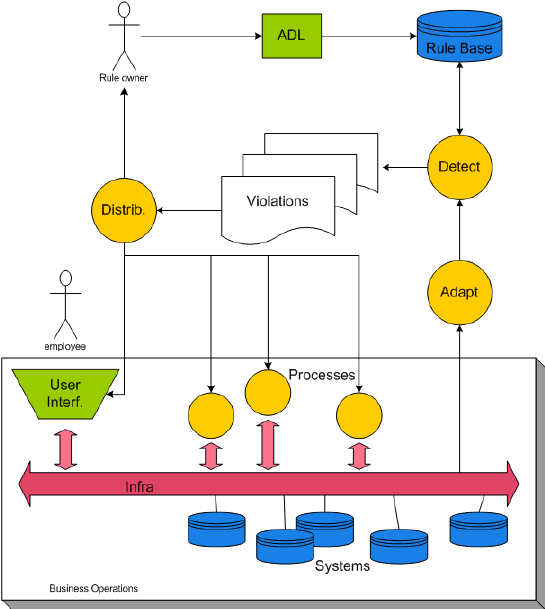
\includegraphics[width=7cm, height=6cm]{Principle-of-rule-based-process-management.png}
\caption{rule-based-proces}
\label{fig:rule-based-proces}
\end{wrapfigure}


The principle of rule-based \acrfull{bpm} as mentioned in \citepNonPub{joosten_joosten} is that any violation of a business rule may be used to trigger actions. 
This is described in the section \nameref{reactive_approach}.

Ampersand consists of concepts that in turn consist of atoms.
An atom is an implementation of the concept.
Inside the \acrshort{big} is a concept "beroep" with associated atoms like "arts, tandarts, etc".
The concepts are given a name, and the name must be recognized by the business.
This also applies to the definition and purpose of the concepts.
These attributes are not mandatory, but when one wants to generate a functional design, these descriptions of the attributes are very useful.
\begin{lstlisting}[language=Octave] 
CONCEPT Beroep "Beroep van een persoon zoals bedoeld in de wet" 
PURPOSE CONCEPT Beroep 
{+Beroep dat uitgeoefend wordt+}
POPULATION Beroep CONTAINS [
    "arts",
    "tandarts",
    "apotheker",
    "gezondheidszorgpsycholoog",
    "psychotherapeut",
    "fysiotherapeut",
    "verloskundige",
    "verpleegkundige",
    "physician assistant",
    "orthopedagoog-generalist"
]
\end{lstlisting}

Concepts can have relationships with each other.
If the data of the concepts is true and the rules yield consistent data then the relationships between real data are facts.
These facts together form one truth.
Not all concepts are directly related.
Within the domain of the \acrshort{big} we could distinguish the concept of "registratie" and the concept of "beroep".
This name is also referred to within ~\citeNonPub{van_wet_2018} in article 3 of \acrshort{big}.
Even the name of the relationship is mentioned in this article, which the legislator calls a "beroepsbeoefenaar".
The law requires that data of the "registratie" be recorded, indicating the corresponding profession (beroep).
In Ampersand, this is modelled as follows.
On the one hand, the "beroep" and also the concept "registratie".
\begin{lstlisting}[language=Octave] 
    CONCEPT Registratie "De registratie van een persoon binnen het register" 
    PURPOSE CONCEPT Registratie 
    {+Vastlegging in het register geeft toegang tot uitoefenen taak binnen de gezondheidszorg+}
\end{lstlisting}
Between the "registratie" and the $persoon$ exists the relationship "beroepsbeoefenaar".
\begin{lstlisting}[language=Octave] 
RELATION beroepsbeoefenaar [Persoon*Registratie] 
MEANING "geregistreerd persoon"
POPULATION beroepsbeoefenaar CONTAINS 
[
  ("Piet",1);
  ("Susan",2);
  ("Gerard",3);
  ("John",4)
]\end{lstlisting}
Also adding the concepts of $persoon$ and $handeling$.
Persons may perform the medical actions, but only when they are qualified.
\begin{lstlisting}[language=Octave] 
    CONCEPT Persoon "Persoon die werkzaam wilt zijn binnen de zorg"
    PURPOSE CONCEPT Persoon 
    {+Vastleggen van de identiteit van de persoon+}
\end{lstlisting}
\begin{lstlisting}[language=Octave] 
    CONCEPT Handeling "Acties die uitgevoerd worden" 
    PURPOSE CONCEPT Handeling 
    {+Vastleggen van de mogelijke handelingen die uitgevoerd kunnen worden binnen de zorg+}
\end{lstlisting}
These concepts can lead us to the following scheme.
\begin{figure}[H] 
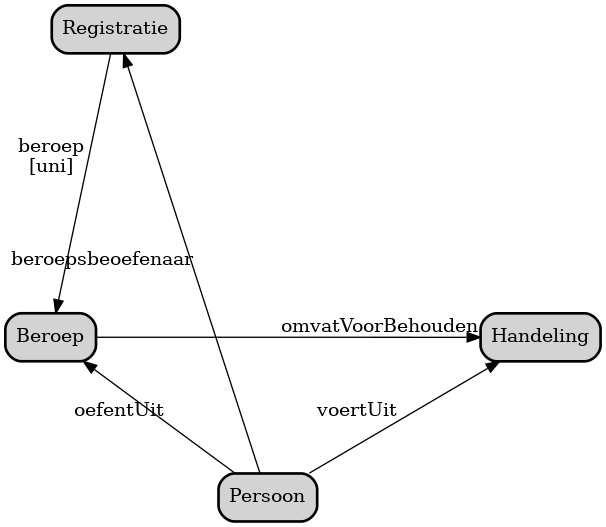
\includegraphics[scale=0.4]{CDConceptBeroep.png}
\centering
\caption{relations}
\label{fig:relations}
\end{figure}
The multiplicity must also be determined for each relation.
\begin{table}[h!]
    \begin{tabular}{||l | l||} 
     \hline
    function & The corresponding control question for the above relation $voerUit$ is\\
    \hline\hline
        Univalent & For each $Persoon$ there is at most 1 $Handeling$\\ %elke P max 1 H
        Total & For each $Persoon$ there is at least 1 $Handeling$ \\ %elke P minimaal 1 H
        Injective & For each $Handeling$ there is only 1 $Persoon$\\ %elke H max 1 P 
        Surjection & For each $Handeling$ there is at least 1 $Persoon$\\ %elke H minimaal 1 P
    \end{tabular}
    \caption{multiplicity}
    \label{tab:multiplicity}
\end{table}

By modelling using the Ampersand method, the question can be answered whether Ampersand provides more insight into the relationships.
As part of the research question, Ampersand can help you gain insight into the relationships.
Although you have to recognize and define these yourself, Ampersand will be helpful in generating functional design and prototype.
The generated prototype will validate the named constraints.
This will prevent registrations that do not meet the constraints.
These constraints are laid down in rules within Ampersand.
For example, a rule can be drawn up that determines whether a person is allowed to perform a certain action.
In figure \ref{fig:relations} the relations are named.
It was previously established that there are 2-tuple relationships.
Here we use the following notation:"$\mathit{relation [Concept \times Concept]}$".
\begin{center}
$\mathit{voertUit [Persoon \times Handeling]}$ ; 
 $\mathit{omvatVoorBehouden [Beroep \times Handeling]~\smallsmile}$
\newline $\subseteq$
\newline $\mathit{beroepsbeoefenaar [persoon \times registratie]}$ ;
$\mathit{beroep [registratie \times beroep]}$
\end{center}
The compared sets are
\newline $\mathit{[Persoon \times Beroep]}$
\newline The rule then will determine if the previous equation is true.
\newline If this is the case, then the rule is validated, otherwise the violation message occurs.
\begin{lstlisting}
    RULE HandelingDoorPersoon: voertUit; omvatVoorBehouden[Beroep*Handeling]~ |- beroepsbeoefenaar; beroep
    MEANING "Een persoon mag handelingen uitvoeren wanneer hij een bepaald beroep uitoefend"
    MESSAGE "Geen toegestane handeling."
    VIOLATION (TXT "Persoon ", SRC I, TXT " voert de handeling uit ", TGT I, TXT " die niet tot zijn beroep behoren ", SRC I[Persoon];oefentUit)
\end{lstlisting}


\subsection{Reactive approach} \label{reactive_approach}

The start of the reactive approach started with the reactive manifesto~\citepNonPub{reactive_manifesto}.
This defines the aspects that a reactive system should meet.
This includes Responsive, Resilient, Elastic and Message Driven.
These are systems that are flexible, loosely coupled and scalable and that makes them easier to develop and maintain.
Reactive Systems are made highly responsive and provide interactive feedback.
\begin{figure}[H] 
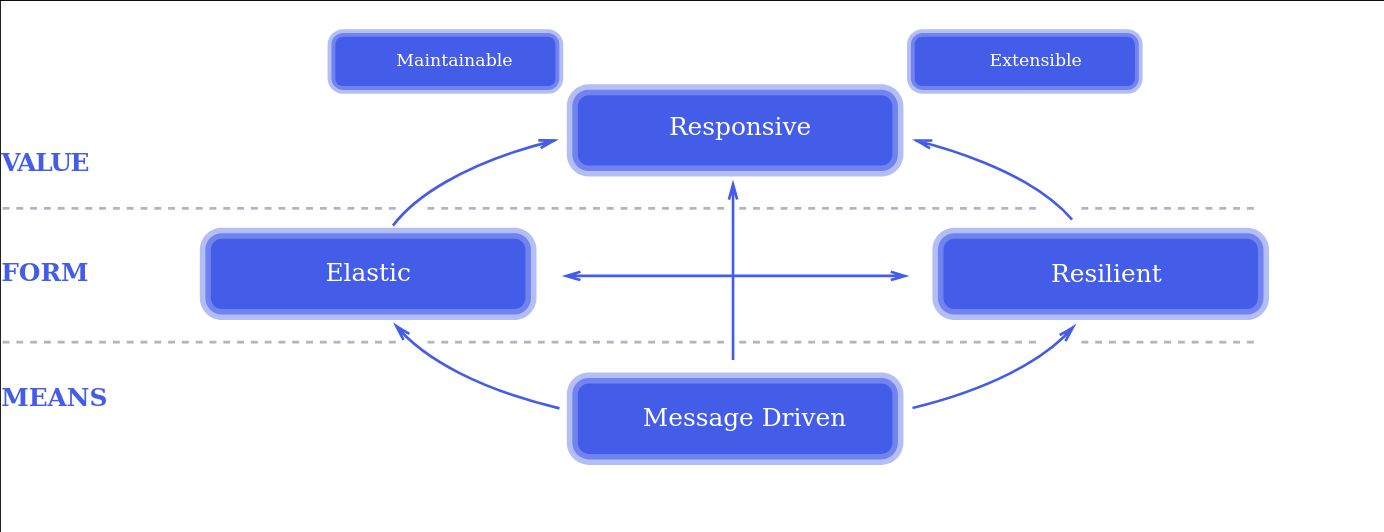
\includegraphics[scale=0.3]{reactive_manifesto.png}
\centering
\caption{reactive manifesto}
\label{fig:reactive manifesto}
\end{figure}


Ampersand is a form of Functional Reactive Programming (FRP)~\citep{elliott_functional_1997}.
The basic of reactive programming is the fact that it involves asynchronous communication.
This means that, as the \citeNonPub{reactive_manifesto} prescribes, use is made of message driven systems, but Ampersand is more than a message-driven system.
It is actually an event-driven system.
The glossary of the \citeNonPub{reactive_manifesto} indicates the difference between message driven systems and event driven systems.
An event-driven system targets event-bus while a message-driven system targets recipients~\citep{bainomugisha_survey_2013}.
The essence is that the order of the flow cannot be determined in advance.
The system will respond to events caused by constraints, Ampersand determines a dynamic flow~\citep{joosten_relation_2018}.




\subsubsection{Law analysis} \label{law_analysis}
The tax authorities have developed a method that is intended to analyse tax laws and other laws.
This is performed in these 6 steps:
\begin{enumerate}
    \item Determining the work area.
    \item Making the structure visible in legislation.
    \item Defining the meaning of legislation.
    \item Validate the analysis results.
    \item Identify missing execution policy.
    \item Setting up the knowledge model.
\end{enumerate}
Emphasis is placed on the cooperation between the implementer, ICT and policy.
By going through the method step by step, one arrives at a shared language.
This shared language includes the definition of concepts by the collaborating parties.
An important part of the approach is dividing the law into small pieces and always refer to these pieces of law in the implementation.
As a result, the method meets the requirement of the justification of government decisions.
The decisions are traceable, explainable, and it is possible to account for them.
What is not clear from the webinar~\citeNonPub{belastingdienst_webinar_2021} is how these steps were converted into an implementation.
The book~\citeNonPub{ausems_wetsanalyse_2021} indicates that the legal analysis method does not contain a development tool, but that the Tax and Customs Administration has developed an instrument based on the legal model, which is not freely available.
\subsection{Design method} \label{design_method}
The method used in this study is the Ampersand method.
The Ampersand method is based on relational algebra.
Ampersand makes it possible to make a conceptual analysis of problems. The data model created thereby makes it possible to accelerate implementation.


\subsubsection{Relation Algebra} \label{relation_algebra}
The field of the relation algebra, founded by De Morgan, focuses on operations with sets.
The signature item of relational algebra is the relationship, as the name implies.
This relationship has several properties, namely the attributes.
The attributes in the example of \acrshort{big} would be the surname, first names, gender, date of birth, nationality and address of the person concerned and the number and time of registration~\footnote{\acrlong{big} article 3, paragraph 2}.
In addition, the relationship consists of tuples.
Since the relationship is always between two objects, this is called 2-tuples.
The tuples contain the attributes of the relation.

Basically the operations on sets are the following:
\begin{itemize}
    \item Union, $R \cup S$ %vereniging
    \item Intersection, $R \cap S$ %doorsnede
    \item Difference, $R - S$ or $S - R$ %verschil
\end{itemize}
A distinction must be made between relation algebra and relational algebra.
Ampersand uses relation algebra, so is tuple related and the relational algebra is the foundation of e.g. relational databases.
This includes projections, selections and joins.
The latter are therefore not part of relation algebra.


\subsubsection{Ampersand} \label{ampersand}
Ampersand is based on relation algebra and focuses on business rules~\citepNonPub{wedemeijer_l_joosten_smm_michels_garkenbout_jlc_werkboek_ontwerpen_met_bedrijfsregelspdf_nodate}.
Ampersand supplies correct information systems.
In this case, Ampersand's goal is to provide a correct registry system.
Ampersand's other strengths are its support for conceptual analysis.
It is a platform for reactive programming and generates prototypes.
Ampersand describes the goals rather than the steps.

Business rules are there to pursue a common goal.
These rules are converted into an information system. 
The Ampersand method ensures that when a precise set of rules has been established, an information system can be generated. 
Ampersand focuses on business rules.
To learn how Ampersand works in real life, we design a registry in Ampersand that implements the \acrshort{big}~\citepNonPub{van_wet_2018} .

\begin{wrapfigure} {r}{0.52\textwidth} 
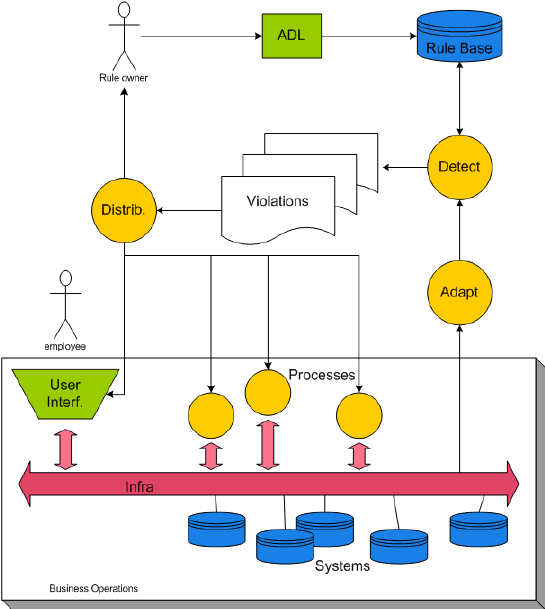
\includegraphics[width=7cm, height=6cm]{Principle-of-rule-based-process-management.png}
\caption{rule-based-proces}
\label{fig:rule-based-proces}
\end{wrapfigure}


The principle of rule-based \acrfull{bpm} as mentioned in \citepNonPub{joosten_joosten} is that any violation of a business rule may be used to trigger actions. 
This is described in the section \nameref{reactive_approach}.

Ampersand consists of concepts that in turn consist of atoms.
An atom is an implementation of the concept.
Inside the \acrshort{big} is a concept "beroep" with associated atoms like "arts, tandarts, etc".
The concepts are given a name, and the name must be recognized by the business.
This also applies to the definition and purpose of the concepts.
These attributes are not mandatory, but when one wants to generate a functional design, these descriptions of the attributes are very useful.
\begin{lstlisting}[language=Octave] 
CONCEPT Beroep "Beroep van een persoon zoals bedoeld in de wet" 
PURPOSE CONCEPT Beroep 
{+Beroep dat uitgeoefend wordt+}
POPULATION Beroep CONTAINS [
    "arts",
    "tandarts",
    "apotheker",
    "gezondheidszorgpsycholoog",
    "psychotherapeut",
    "fysiotherapeut",
    "verloskundige",
    "verpleegkundige",
    "physician assistant",
    "orthopedagoog-generalist"
]
\end{lstlisting}

Concepts can have relationships with each other.
If the data of the concepts is true and the rules yield consistent data then the relationships between real data are facts.
These facts together form one truth.
Not all concepts are directly related.
Within the domain of the \acrshort{big} we could distinguish the concept of "registratie" and the concept of "beroep".
This name is also referred to within ~\citeNonPub{van_wet_2018} in article 3 of \acrshort{big}.
Even the name of the relationship is mentioned in this article, which the legislator calls a "beroepsbeoefenaar".
The law requires that data of the "registratie" be recorded, indicating the corresponding profession (beroep).
In Ampersand, this is modelled as follows.
On the one hand, the "beroep" and also the concept "registratie".
\begin{lstlisting}[language=Octave] 
    CONCEPT Registratie "De registratie van een persoon binnen het register" 
    PURPOSE CONCEPT Registratie 
    {+Vastlegging in het register geeft toegang tot uitoefenen taak binnen de gezondheidszorg+}
\end{lstlisting}
Between the "registratie" and the $persoon$ exists the relationship "beroepsbeoefenaar".
\begin{lstlisting}[language=Octave] 
RELATION beroepsbeoefenaar [Persoon*Registratie] 
MEANING "geregistreerd persoon"
POPULATION beroepsbeoefenaar CONTAINS 
[
  ("Piet",1);
  ("Susan",2);
  ("Gerard",3);
  ("John",4)
]\end{lstlisting}
Also adding the concepts of $persoon$ and $handeling$.
Persons may perform the medical actions, but only when they are qualified.
\begin{lstlisting}[language=Octave] 
    CONCEPT Persoon "Persoon die werkzaam wilt zijn binnen de zorg"
    PURPOSE CONCEPT Persoon 
    {+Vastleggen van de identiteit van de persoon+}
\end{lstlisting}
\begin{lstlisting}[language=Octave] 
    CONCEPT Handeling "Acties die uitgevoerd worden" 
    PURPOSE CONCEPT Handeling 
    {+Vastleggen van de mogelijke handelingen die uitgevoerd kunnen worden binnen de zorg+}
\end{lstlisting}
These concepts can lead us to the following scheme.
\begin{figure}[H] 
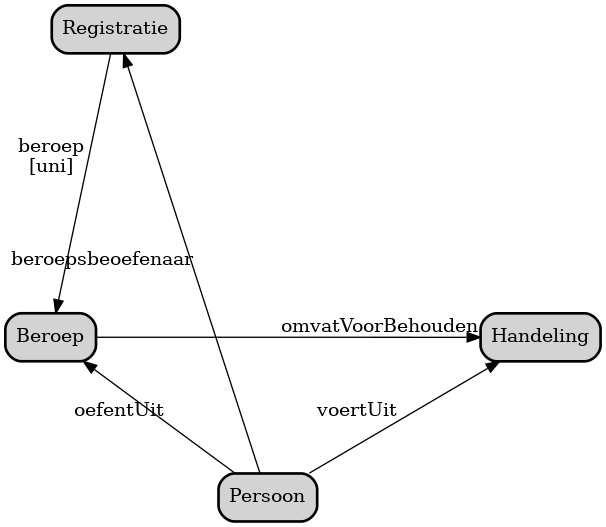
\includegraphics[scale=0.4]{CDConceptBeroep.png}
\centering
\caption{relations}
\label{fig:relations}
\end{figure}
The multiplicity must also be determined for each relation.
\begin{table}[h!]
    \begin{tabular}{||l | l||} 
     \hline
    function & The corresponding control question for the above relation $voerUit$ is\\
    \hline\hline
        Univalent & For each $Persoon$ there is at most 1 $Handeling$\\ %elke P max 1 H
        Total & For each $Persoon$ there is at least 1 $Handeling$ \\ %elke P minimaal 1 H
        Injective & For each $Handeling$ there is only 1 $Persoon$\\ %elke H max 1 P 
        Surjection & For each $Handeling$ there is at least 1 $Persoon$\\ %elke H minimaal 1 P
    \end{tabular}
    \caption{multiplicity}
    \label{tab:multiplicity}
\end{table}

By modelling using the Ampersand method, the question can be answered whether Ampersand provides more insight into the relationships.
As part of the research question, Ampersand can help you gain insight into the relationships.
Although you have to recognize and define these yourself, Ampersand will be helpful in generating functional design and prototype.
The generated prototype will validate the named constraints.
This will prevent registrations that do not meet the constraints.
These constraints are laid down in rules within Ampersand.
For example, a rule can be drawn up that determines whether a person is allowed to perform a certain action.
In figure \ref{fig:relations} the relations are named.
It was previously established that there are 2-tuple relationships.
Here we use the following notation:"$\mathit{relation [Concept \times Concept]}$".
\begin{center}
$\mathit{voertUit [Persoon \times Handeling]}$ ; 
 $\mathit{omvatVoorBehouden [Beroep \times Handeling]~\smallsmile}$
\newline $\subseteq$
\newline $\mathit{beroepsbeoefenaar [persoon \times registratie]}$ ;
$\mathit{beroep [registratie \times beroep]}$
\end{center}
The compared sets are
\newline $\mathit{[Persoon \times Beroep]}$
\newline The rule then will determine if the previous equation is true.
\newline If this is the case, then the rule is validated, otherwise the violation message occurs.
\begin{lstlisting}
    RULE HandelingDoorPersoon: voertUit; omvatVoorBehouden[Beroep*Handeling]~ |- beroepsbeoefenaar; beroep
    MEANING "Een persoon mag handelingen uitvoeren wanneer hij een bepaald beroep uitoefend"
    MESSAGE "Geen toegestane handeling."
    VIOLATION (TXT "Persoon ", SRC I, TXT " voert de handeling uit ", TGT I, TXT " die niet tot zijn beroep behoren ", SRC I[Persoon];oefentUit)
\end{lstlisting}


\subsection{Reactive approach} \label{reactive_approach}

The start of the reactive approach started with the reactive manifesto~\citepNonPub{reactive_manifesto}.
This defines the aspects that a reactive system should meet.
This includes Responsive, Resilient, Elastic and Message Driven.
These are systems that are flexible, loosely coupled and scalable and that makes them easier to develop and maintain.
Reactive Systems are made highly responsive and provide interactive feedback.
\begin{figure}[H] 
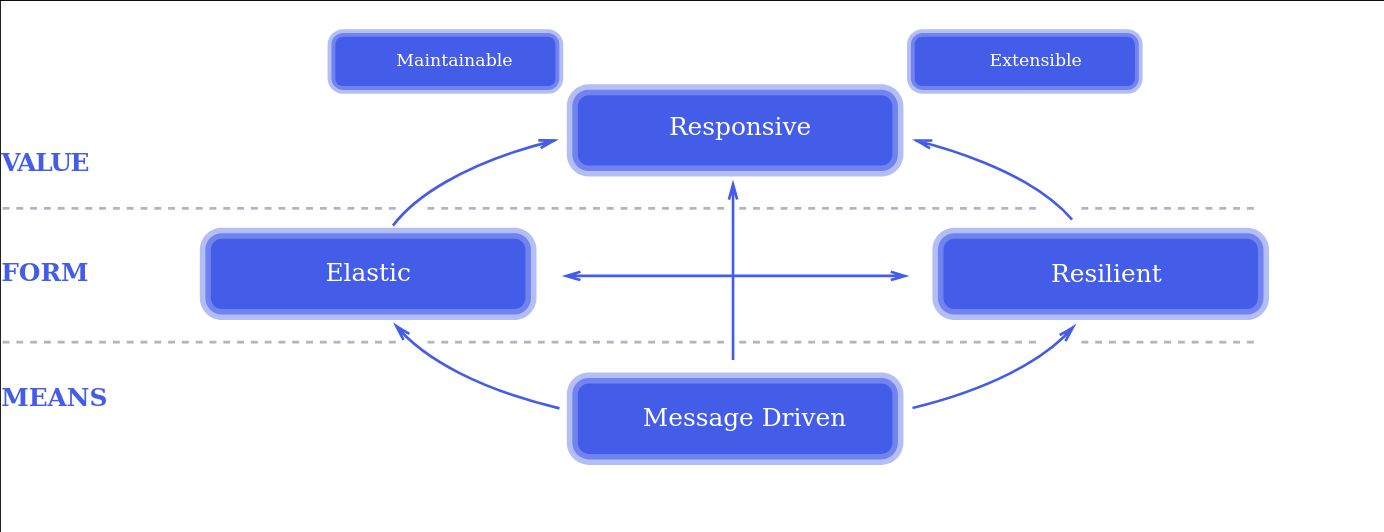
\includegraphics[scale=0.3]{reactive_manifesto.png}
\centering
\caption{reactive manifesto}
\label{fig:reactive manifesto}
\end{figure}


Ampersand is a form of Functional Reactive Programming (FRP)~\citep{elliott_functional_1997}.
The basic of reactive programming is the fact that it involves asynchronous communication.
This means that, as the \citeNonPub{reactive_manifesto} prescribes, use is made of message driven systems, but Ampersand is more than a message-driven system.
It is actually an event-driven system.
The glossary of the \citeNonPub{reactive_manifesto} indicates the difference between message driven systems and event driven systems.
An event-driven system targets event-bus while a message-driven system targets recipients~\citep{bainomugisha_survey_2013}.
The essence is that the order of the flow cannot be determined in advance.
The system will respond to events caused by constraints, Ampersand determines a dynamic flow~\citep{joosten_relation_2018}.




\subsubsection{Law analysis} \label{law_analysis}
The tax authorities have developed a method that is intended to analyse tax laws and other laws.
This is performed in these 6 steps:
\begin{enumerate}
    \item Determining the work area.
    \item Making the structure visible in legislation.
    \item Defining the meaning of legislation.
    \item Validate the analysis results.
    \item Identify missing execution policy.
    \item Setting up the knowledge model.
\end{enumerate}
Emphasis is placed on the cooperation between the implementer, ICT and policy.
By going through the method step by step, one arrives at a shared language.
This shared language includes the definition of concepts by the collaborating parties.
An important part of the approach is dividing the law into small pieces and always refer to these pieces of law in the implementation.
As a result, the method meets the requirement of the justification of government decisions.
The decisions are traceable, explainable, and it is possible to account for them.
What is not clear from the webinar~\citeNonPub{belastingdienst_webinar_2021} is how these steps were converted into an implementation.
The book~\citeNonPub{ausems_wetsanalyse_2021} indicates that the legal analysis method does not contain a development tool, but that the Tax and Customs Administration has developed an instrument based on the legal model, which is not freely available.

\newpage
\section{Conclusions and Future work} \label{Conclusions}

\subsection{Conclusions}\label{conclusions}

In this research we investigated how useful Ampersand is for designing registry systems by analyzing legislation and regulations.
We did this in the form of \acrshort{ar} and the case used is the \acrshort{big}.

The Ampersand method was used to analyze part of the law and to process it via scripting (see appendix~\ref{appendixAdl}) into a prototype (see appendix~\ref{appendixPrototype}) and \acrlong{ca} ( see appendix~\ref{ConceptualAnalysis}).
During the analysis phase, observations (see appendix~\ref{appendixLoglines}) were made.
These are recorded with date and time stamp.
In addition to the analysis, there were interviews (see appendix~\ref{appendixInterviews}) with a number of people from the \acrshort{cibg} organization.
During the interviews the Ampersand approach was discussed and the \acrlong{ca} and the prototype were discussed.
The collected data from observations and interview has been input for the content analysis (see appendix~\ref{appendixContentAnalysis}).

In addition to the main question "\acrlong{research question}" sub-questions have been defined. 
The sub-questions contribute to answering the main question.
The parts of this question are discussed in subsection~\ref{subsection:ampersand-knowledge}.

\subsubsection{Engineering perspective}\label{subsub:engineering_perspective}
The knowledge that the software engineer needs to be able to work with Ampersand is not limited to the knowledge of Ampersand.
Due to the setup of Ampersand, it was eventually set up in Docker, after we experimented with a RAP environment on the server of \acrlong{ou} and later a local environment in \acrshort{x}.
We need knowledge about the design, use and operation of Docker.

\acrlong{ra} is used to establish relationships between Concepts and to compose the Rules.
Knowledge of Relation Algebra in combination with Ampersand can be gained by following the Rule-Based Design course of the \acrshort{ou}, or at least by reading the accompanying book.

Once Ampersand its knowledge has been acquired, through theory and practice, it is important to keep this knowledge up to date.
Ampersand its application knowledge should now be available on the Internet, at sites like \url{https://stackoverflow.com} and other trusted information sites.
Due to a small community and, as noted earlier, low usage, application knowledge on the internet is very limited.
To build a readable \acrlong{ca} we use the scripts from Ampersand.

For the \acrlong{ca} we use the Include statements to control the build.
Best practices should be collected to simplify the start of an Ampersand project.

When performing the analysis, there is a need for overview.
On the one hand, an overview of the treatment of the source document, because it is necessary to keep track of which parts of the legal texts have already been processed and which have not yet been processed.
For this you need an annotation tool, which helps you to record the processing and helps you to keep the overview.

On the other hand, an overview is also needed while creating the script to be able to refactor things and avoid duplication.
There is a tool for this called Atlas, but it is only available in the RAP environment and not in the local setup.

Ampersand has built in a form of authorization that works through Rules and on the Interfaces.
With this authorization, a distinction can be made between user roles and the applications that are allowed to run in the prototype.

Knowledge is also required about dealing with shared Concepts.
Sharing can relate to Concepts within one project, sharing or reusing, as in the case, generic patterns with associated Concepts.
This form of sharing works if all components are deployed simultaneously, but it is then not possible to run different non-generic components side by side (see figure~\ref{fig:arts-deploy}, \ref{fig:tandarts-deploy} and \ref{fig:monoliet-deployment}).
The foregoing concerns the sharing of Concepts within a project.

Connections must be made to existing Concepts, which are not always called Concepts, within the organization.
The mapping between the Concepts found and the existing ones, with which the Ampersand implementation has a relationship, must be performed.

Another form of sharing Concepts concerns projects.
Defined concepts included in Patterns will be reused by other projects.

The prototype is an HTML website in combination with CSS.
When changes are made to this, knowledge of HTML and CSS is required.
The extra functions that are not (yet) in Ampersand can be made in PHP.
So using this requires knowledge of PHP.

\subsubsection{Components perspective}\label{subsub:components_perspective}
The question about Concepts, Relations and Rules, which appear in the \acrshort{big}, can be referred to the appendix~\ref{ConceptualAnalysis}.
Here we find an overview of all these elements.

A finding that emerges here concerns the embedding in the software architecture of the ICT organization.
In the software architecture, the software components are managed and there is an overview of the relationships between these components.
We can see the subsystems or patterns found as software components.
It then appears that there is a certain overlap of Concepts and Relations in the existing architecture and the model that Ampersand has made.
A very careful analysis is needed to discover this overlap.
The name of a Concept or Relation does not have to match, but the meaning does.
It is also possible that the naming matches, but the meaning does not.

In short, the existing software landscape needs to be carefully examined to determine which parts of the Ampersand model can be implemented

For the legal registers, no agreements in the form of data may be shared, so no data reuse.
For example, the customer in the Donor Register may never be linked to a BIG registration for the purpose of reusing customer data.

\subsubsection{Laws perspective}\label{subsub:laws_perspective}
With the question of the usability of the law for the Ampersand method, the aspects are named in subsection~\ref{subsection:setup-law-for-ampersand}.

We chose the \acrshort{big} to analyze with the Ampersand method.
This law was chosen because there was a need from \acrshort{cibg} to redesign and build the system that supports the law.
With Ampersand we are going to do part of the redesign.

During the analysis phase, we encountered a number of issues that do not support the choice of law and that a later choice of law should preferably comply with.
For example, the law appears to be ambiguous on some points, according to the lawyer.

Experience with law is necessary to be able to analyze law properly.
This is especially true if the law, such as \acrshort{big}, has options for interpretation.

The age of the original law may give rise to interpretation.
The complexity and scope of the law makes the analysis less straightforward.

When we start with the legal analysis, a team consists of at least one lawyer and two analysts.
This guarantees legal knowledge and experience in reading and interpreting laws and regulations.
The analysts have to keep each other on their toes when making the \acrlong{ca}.

At the start, we map out all relevant legislation and regulations and determine which legislation is included in the analysis.
After the step, the structure is determined for each part and we probably have an idea of what the system can look like.
We assume here that the structure of the analysis will follow the structure of the law.

We can do the analysis of the law, even though this law is ambiguous, complex, old and large, but it does make the journey difficult.
One way is to be closer to the legislature so that he is already aware of the writing of the law and is considering the translation of the law into a registry system.
One idea is that the law would already be designed directly in \acrshort{ra}.
The formal approach makes it completely clear what the law complies with.

This just goes to show why it is necessary to work with a lawyer.
The lawyer can interpret the law and knows how to navigate the law.

\subsubsection{Organization perspective}\label{subsub:organization_perspective}
What are the strengths and weaknesses of using Ampersand for registry systems in a government organization.
We can say that the analysis of a law can lead to a register system and because it is a register system, which is derived from the law, it will always be placed with a government organization.
We also concluded that there are not many observations and comments about registry systems.
Then it remains to map the strengths and weaknesses of Ampersand for a government organization and then specifically for the \acrshort{cibg}.
From the perspective of weakness and strength we will go through all parts.

API availability at Ampersand at the prototype stage and many systems use APIs to communicate with the source.
The description of the APIs are missing and can be retrieved from the log.
Pushing the description of the APIs to Swagger, for example, makes it easier to use the APIs.
Adapting response from the API to the calling system would be an improvement.

The mapping from Ampersand Concepts to \acrshort{rk} is performed so that Ampersand analysis connects to \acrshort{rk}, thereby integration takes place.
This is a manual operation and can cause errors such that incorrect mappings take place or mapping does not take place.

The \acrshort{rk} has a customization that makes it possible to place register values in the editable part.
The mapping and customization will bring Ampersand and \acrshort{rk} closer together.

The issue of maintenance on the Ampersand model has been discussed before.
A strong point here is that after every maintenance a completely new model is created and no technical debt is introduced, but by always setting up a completely new system, it is now not possible to migrate the data.
Ampersand systems are not used live, so the data conversion is only needed for the prototype environment.

Ampersand is a reactive designed system.
The business rules actually define the process.
The tool generates error-free specifications to support the business process.
The \acrshort{cibg} is a strong process oriented organization.

The analyst needs an overview when managing the Concepts, Relations and Rules.
Within RAP, the Atlas tool is available for this, but not for the local environment.
We were working with an Excel sheet during the research, but this results in duplication of records and problems.
Within the IDE, for example IntelIJ, programming languages have refactoring tools.
We have been working with \acrshort{vsc}, here the refactoring was not present and it happened that this caused inconsistency and the compilation did not run correctly.

The \acrlong{ca} is created as deliverable.
This is used as a design for the implementation and because it is available early in the process, it can also be used as a validation tool and to base tests on.
The prototype can also be used as a test basis and real tests can be performed on this.
In combination with the API, the prototype can act in whole or in part as a stub.

For an organisation, a new method can be experienced as threatening~\citep{antons_assessing_2017}.
It is therefore possible that one reacts with an NIH action.
To deal with this, it is wise to conduct an extensive POC and actively inform the parties.
Assemble a team and use them as promoters.
Non-ICT professionals can also be deployed as Ampersand modellers within the team, provided they have knowledge of Relation Algebra.

Ampersand should get a little more exposure than it is now just in the scientific environment.
The more it is known, the more it is used, making it more famous again.
Now there is a certain reluctance to use and that has the basis in the obscurity of Ampersand.

Overall conclusion is that Ampersand is a useful product for translating the law.
The output products are very useful for the \acrshort{cibg}.
Not all laws are equally suitable and the application of Ampersand in the development process must be incorporated.
The latter still requires some mission work because it is different from what people are used to and it is very unknown.
An organization will have to focus on using this and the organization \acrshort{cibg} is not very change-oriented.

\subsection{Future work}\label{future_work}
Now that the research has been completed and the results and conclusions have been described, it is worth considering what further research could take place.
The conclusions revealed that there are omissions in the area of maintaining an overview.
In future research, attention could be given to the way in which this overview can be maintained.
This may move in the direction of annotation tools.
The follow-up research could focus on selecting and implementing tools within Ampersand for the purpose of maintaining overview.
An overview is also needed on the Concepts management side.
This seems to be possible by porting Atlas from RAP to the local environment.

In the context of maintaining the overview, it has been suggested to make use of the addition of XML in the source document.
So enriching the source document with the annotation XML.
The big advantage of this would be that it is then possible to generate the Ampersand script.
Especially after changes in the source document, where the existing annotations can be inserted in the new version.
This adjustment would be even more beneficial once there is an existing national base of Concepts and Relations.
The link between annotations and the national base could result in an enormous acceleration in development.
This is worth investigating, but will have to be split into several studies.

Another conclusion that has been drawn is that the \acrshort{big} is not the most suitable law to analyze it via the Ampersand method.
This is not the fault of Ampersand, but the law.
It is interesting to map out which requirements the law must meet in order to fit in well with the method and the follow-up is to examine how we can shape future laws that people would like to be supported by (register) systems so that they can be quickly analyzed by Ampersand.
Early participation by business analyst and Ampersand skilled lawyers in the legislative process could save a lot of time and money.
How much that may be is a topic for a research project.

One of the interviewees feared that the Ampersand approach would take more time in the design phase than the regular approach.
The regular approach includes a more or less agile approach, in which the design is made in outline, after which the system is divided into parts and these are made agile.
One could examine the design of two similar systems or possibly even the same system, with one done the Ampersand way and the other the regular way.
Then it is interesting to see what is faster, more complete and more workable for the follow-up process.

Another comment made during the interviews relates to the size of the system.
The hypothesis was that the system size of an Ampersand project will be smaller than the size of a system from a regular trajectory.
This could be related to the fact that Ampersand is directly on the source and does not want to include all kinds of peripheral matters.

During the research we were regularly confronted with the \acrshort{rk}.
It is worth investigating how exactly this link should be established.
Where are the similarities and where are the differences?
In this context we again come across the issue of the common Concepts.

To ensure a smooth start of a project, it is good to start from a standard set of agreements.
Let us develop best practices, including things like naming (upper and lower case, CamelCase, etc.) and suggestions regarding the use of source texts.
So that these can be used at the kick-off of an Ampersand project.






\newpage
\section{Reflection} \label{reflection}

TODO

\subsection{Design method} \label{design_method}
The method used in this study is the Ampersand method.
The Ampersand method is based on relational algebra.
Ampersand makes it possible to make a conceptual analysis of problems. The data model created thereby makes it possible to accelerate implementation.


\subsubsection{Relation Algebra} \label{relation_algebra}
The field of the relation algebra, founded by De Morgan, focuses on operations with sets.
The signature item of relational algebra is the relationship, as the name implies.
This relationship has several properties, namely the attributes.
The attributes in the example of \acrshort{big} would be the surname, first names, gender, date of birth, nationality and address of the person concerned and the number and time of registration~\footnote{\acrlong{big} article 3, paragraph 2}.
In addition, the relationship consists of tuples.
Since the relationship is always between two objects, this is called 2-tuples.
The tuples contain the attributes of the relation.

Basically the operations on sets are the following:
\begin{itemize}
    \item Union, $R \cup S$ %vereniging
    \item Intersection, $R \cap S$ %doorsnede
    \item Difference, $R - S$ or $S - R$ %verschil
\end{itemize}
A distinction must be made between relation algebra and relational algebra.
Ampersand uses relation algebra, so is tuple related and the relational algebra is the foundation of e.g. relational databases.
This includes projections, selections and joins.
The latter are therefore not part of relation algebra.


\subsubsection{Ampersand} \label{ampersand}
Ampersand is based on relation algebra and focuses on business rules~\citepNonPub{wedemeijer_l_joosten_smm_michels_garkenbout_jlc_werkboek_ontwerpen_met_bedrijfsregelspdf_nodate}.
Ampersand supplies correct information systems.
In this case, Ampersand's goal is to provide a correct registry system.
Ampersand's other strengths are its support for conceptual analysis.
It is a platform for reactive programming and generates prototypes.
Ampersand describes the goals rather than the steps.

Business rules are there to pursue a common goal.
These rules are converted into an information system. 
The Ampersand method ensures that when a precise set of rules has been established, an information system can be generated. 
Ampersand focuses on business rules.
To learn how Ampersand works in real life, we design a registry in Ampersand that implements the \acrshort{big}~\citepNonPub{van_wet_2018} .

\begin{wrapfigure} {r}{0.52\textwidth} 
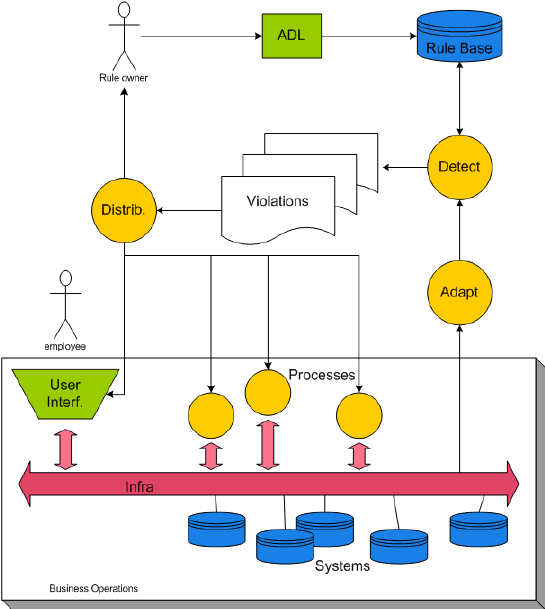
\includegraphics[width=7cm, height=6cm]{Principle-of-rule-based-process-management.png}
\caption{rule-based-proces}
\label{fig:rule-based-proces}
\end{wrapfigure}


The principle of rule-based \acrfull{bpm} as mentioned in \citepNonPub{joosten_joosten} is that any violation of a business rule may be used to trigger actions. 
This is described in the section \nameref{reactive_approach}.

Ampersand consists of concepts that in turn consist of atoms.
An atom is an implementation of the concept.
Inside the \acrshort{big} is a concept "beroep" with associated atoms like "arts, tandarts, etc".
The concepts are given a name, and the name must be recognized by the business.
This also applies to the definition and purpose of the concepts.
These attributes are not mandatory, but when one wants to generate a functional design, these descriptions of the attributes are very useful.
\begin{lstlisting}[language=Octave] 
CONCEPT Beroep "Beroep van een persoon zoals bedoeld in de wet" 
PURPOSE CONCEPT Beroep 
{+Beroep dat uitgeoefend wordt+}
POPULATION Beroep CONTAINS [
    "arts",
    "tandarts",
    "apotheker",
    "gezondheidszorgpsycholoog",
    "psychotherapeut",
    "fysiotherapeut",
    "verloskundige",
    "verpleegkundige",
    "physician assistant",
    "orthopedagoog-generalist"
]
\end{lstlisting}

Concepts can have relationships with each other.
If the data of the concepts is true and the rules yield consistent data then the relationships between real data are facts.
These facts together form one truth.
Not all concepts are directly related.
Within the domain of the \acrshort{big} we could distinguish the concept of "registratie" and the concept of "beroep".
This name is also referred to within ~\citeNonPub{van_wet_2018} in article 3 of \acrshort{big}.
Even the name of the relationship is mentioned in this article, which the legislator calls a "beroepsbeoefenaar".
The law requires that data of the "registratie" be recorded, indicating the corresponding profession (beroep).
In Ampersand, this is modelled as follows.
On the one hand, the "beroep" and also the concept "registratie".
\begin{lstlisting}[language=Octave] 
    CONCEPT Registratie "De registratie van een persoon binnen het register" 
    PURPOSE CONCEPT Registratie 
    {+Vastlegging in het register geeft toegang tot uitoefenen taak binnen de gezondheidszorg+}
\end{lstlisting}
Between the "registratie" and the $persoon$ exists the relationship "beroepsbeoefenaar".
\begin{lstlisting}[language=Octave] 
RELATION beroepsbeoefenaar [Persoon*Registratie] 
MEANING "geregistreerd persoon"
POPULATION beroepsbeoefenaar CONTAINS 
[
  ("Piet",1);
  ("Susan",2);
  ("Gerard",3);
  ("John",4)
]\end{lstlisting}
Also adding the concepts of $persoon$ and $handeling$.
Persons may perform the medical actions, but only when they are qualified.
\begin{lstlisting}[language=Octave] 
    CONCEPT Persoon "Persoon die werkzaam wilt zijn binnen de zorg"
    PURPOSE CONCEPT Persoon 
    {+Vastleggen van de identiteit van de persoon+}
\end{lstlisting}
\begin{lstlisting}[language=Octave] 
    CONCEPT Handeling "Acties die uitgevoerd worden" 
    PURPOSE CONCEPT Handeling 
    {+Vastleggen van de mogelijke handelingen die uitgevoerd kunnen worden binnen de zorg+}
\end{lstlisting}
These concepts can lead us to the following scheme.
\begin{figure}[H] 
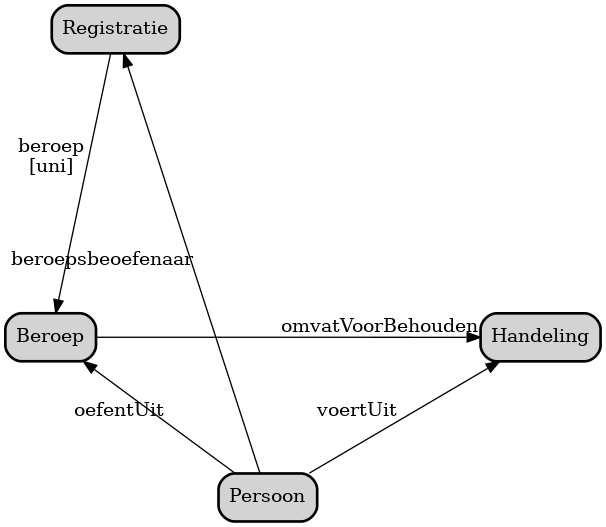
\includegraphics[scale=0.4]{CDConceptBeroep.png}
\centering
\caption{relations}
\label{fig:relations}
\end{figure}
The multiplicity must also be determined for each relation.
\begin{table}[h!]
    \begin{tabular}{||l | l||} 
     \hline
    function & The corresponding control question for the above relation $voerUit$ is\\
    \hline\hline
        Univalent & For each $Persoon$ there is at most 1 $Handeling$\\ %elke P max 1 H
        Total & For each $Persoon$ there is at least 1 $Handeling$ \\ %elke P minimaal 1 H
        Injective & For each $Handeling$ there is only 1 $Persoon$\\ %elke H max 1 P 
        Surjection & For each $Handeling$ there is at least 1 $Persoon$\\ %elke H minimaal 1 P
    \end{tabular}
    \caption{multiplicity}
    \label{tab:multiplicity}
\end{table}

By modelling using the Ampersand method, the question can be answered whether Ampersand provides more insight into the relationships.
As part of the research question, Ampersand can help you gain insight into the relationships.
Although you have to recognize and define these yourself, Ampersand will be helpful in generating functional design and prototype.
The generated prototype will validate the named constraints.
This will prevent registrations that do not meet the constraints.
These constraints are laid down in rules within Ampersand.
For example, a rule can be drawn up that determines whether a person is allowed to perform a certain action.
In figure \ref{fig:relations} the relations are named.
It was previously established that there are 2-tuple relationships.
Here we use the following notation:"$\mathit{relation [Concept \times Concept]}$".
\begin{center}
$\mathit{voertUit [Persoon \times Handeling]}$ ; 
 $\mathit{omvatVoorBehouden [Beroep \times Handeling]~\smallsmile}$
\newline $\subseteq$
\newline $\mathit{beroepsbeoefenaar [persoon \times registratie]}$ ;
$\mathit{beroep [registratie \times beroep]}$
\end{center}
The compared sets are
\newline $\mathit{[Persoon \times Beroep]}$
\newline The rule then will determine if the previous equation is true.
\newline If this is the case, then the rule is validated, otherwise the violation message occurs.
\begin{lstlisting}
    RULE HandelingDoorPersoon: voertUit; omvatVoorBehouden[Beroep*Handeling]~ |- beroepsbeoefenaar; beroep
    MEANING "Een persoon mag handelingen uitvoeren wanneer hij een bepaald beroep uitoefend"
    MESSAGE "Geen toegestane handeling."
    VIOLATION (TXT "Persoon ", SRC I, TXT " voert de handeling uit ", TGT I, TXT " die niet tot zijn beroep behoren ", SRC I[Persoon];oefentUit)
\end{lstlisting}


\subsection{Reactive approach} \label{reactive_approach}

The start of the reactive approach started with the reactive manifesto~\citepNonPub{reactive_manifesto}.
This defines the aspects that a reactive system should meet.
This includes Responsive, Resilient, Elastic and Message Driven.
These are systems that are flexible, loosely coupled and scalable and that makes them easier to develop and maintain.
Reactive Systems are made highly responsive and provide interactive feedback.
\begin{figure}[H] 
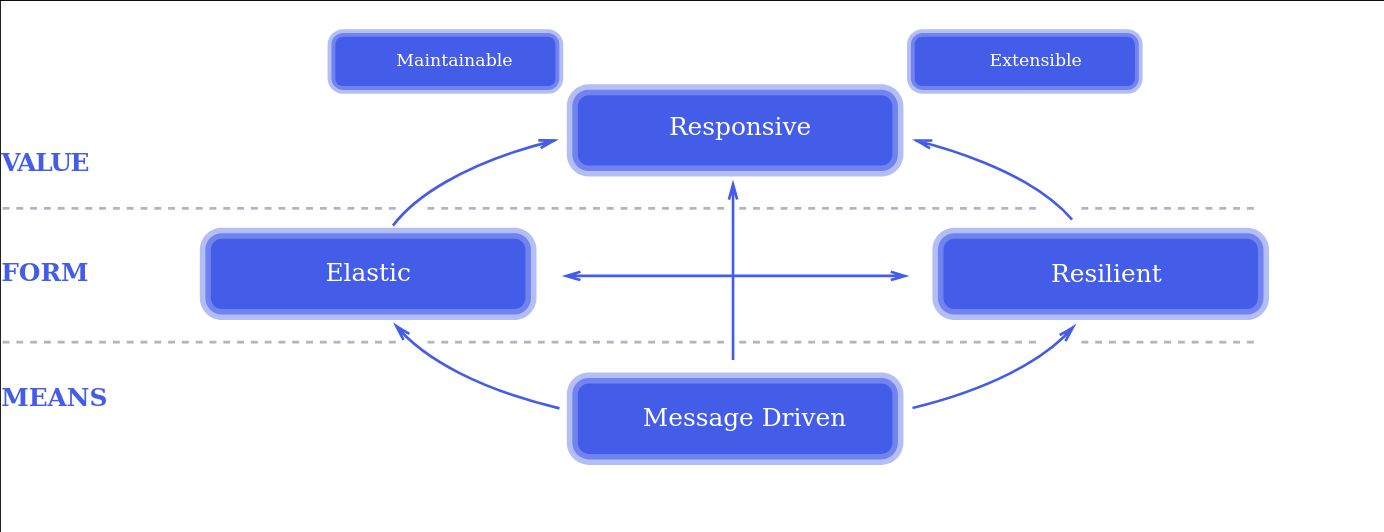
\includegraphics[scale=0.3]{reactive_manifesto.png}
\centering
\caption{reactive manifesto}
\label{fig:reactive manifesto}
\end{figure}


Ampersand is a form of Functional Reactive Programming (FRP)~\citep{elliott_functional_1997}.
The basic of reactive programming is the fact that it involves asynchronous communication.
This means that, as the \citeNonPub{reactive_manifesto} prescribes, use is made of message driven systems, but Ampersand is more than a message-driven system.
It is actually an event-driven system.
The glossary of the \citeNonPub{reactive_manifesto} indicates the difference between message driven systems and event driven systems.
An event-driven system targets event-bus while a message-driven system targets recipients~\citep{bainomugisha_survey_2013}.
The essence is that the order of the flow cannot be determined in advance.
The system will respond to events caused by constraints, Ampersand determines a dynamic flow~\citep{joosten_relation_2018}.




\subsubsection{Law analysis} \label{law_analysis}
The tax authorities have developed a method that is intended to analyse tax laws and other laws.
This is performed in these 6 steps:
\begin{enumerate}
    \item Determining the work area.
    \item Making the structure visible in legislation.
    \item Defining the meaning of legislation.
    \item Validate the analysis results.
    \item Identify missing execution policy.
    \item Setting up the knowledge model.
\end{enumerate}
Emphasis is placed on the cooperation between the implementer, ICT and policy.
By going through the method step by step, one arrives at a shared language.
This shared language includes the definition of concepts by the collaborating parties.
An important part of the approach is dividing the law into small pieces and always refer to these pieces of law in the implementation.
As a result, the method meets the requirement of the justification of government decisions.
The decisions are traceable, explainable, and it is possible to account for them.
What is not clear from the webinar~\citeNonPub{belastingdienst_webinar_2021} is how these steps were converted into an implementation.
The book~\citeNonPub{ausems_wetsanalyse_2021} indicates that the legal analysis method does not contain a development tool, but that the Tax and Customs Administration has developed an instrument based on the legal model, which is not freely available.

\newpage
\newpage
\printglossary[type=\acronymtype]

%\nocite{*}
\bibliographystyle{plainnat}
\bibliographystyleNonPub{plainnat}
\bibliography{report}
\bibliographyNonPub{reportNonPub}


\end{document}




